\documentclass[aspectratio=169]{beamer}

\usetheme{default}
\setbeamertemplate{navigation symbols}{}
\setbeamertemplate{enumerate item}{\color{navy}\arabic{enumi}.}
\setbeamertemplate{itemize item}{\color{black}\textbullet}
\setbeamertemplate{itemize subitem}{\color{black}\textbullet}
\usepackage{booktabs}
\usepackage{xcolor}
\usepackage{tikz}
\usetikzlibrary{shapes,arrows,positioning}
\definecolor{navy}{RGB}{0, 0, 128}
\definecolor{lightblue}{RGB}{230,240,250}
\definecolor{darkgreen}{RGB}{0,100,0}
\definecolor{lightgreen}{RGB}{230,250,230}
\newcommand{\highlight}[1]{\colorbox{lightblue}{$\displaystyle\textcolor{navy}{#1}$}}
\newcommand{\highlighttext}[1]{\colorbox{lightblue}{\textcolor{navy}{#1}}}
\newcommand{\highlightgreen}[1]{\colorbox{lightgreen}{$\displaystyle\textcolor{darkgreen}{#1}$}}

\begin{document}

\begin{frame}

Hotz \& Miller (1993): terminal actions

\bigskip\par

Rust (1987): renewal actions

\bigskip\par

\onslide<2->{
What if no such actions exist?
\bigskip\par
}

\begin{itemize}
\itemsep1.5em
    \item<3-> CCPs still work, but need additional terms beyond $\log p_{kt+1}$ 
    \item<4-> Also likely need additional assumptions about how states evolve
\end{itemize}

\onslide<5->{
\bigskip\par
\textcolor{navy}{Finite dependence}: when $V_{t+\tau}$ terms cancel after $\tau$ (finite number) periods ahead
\bigskip\par
}

\begin{itemize}
\itemsep1.5em
    \item<6-> Typically can get models where $\tau=3$, meaning only need 2-period-ahead CCPs
\end{itemize}
\end{frame}




\begin{frame}

\begin{center}
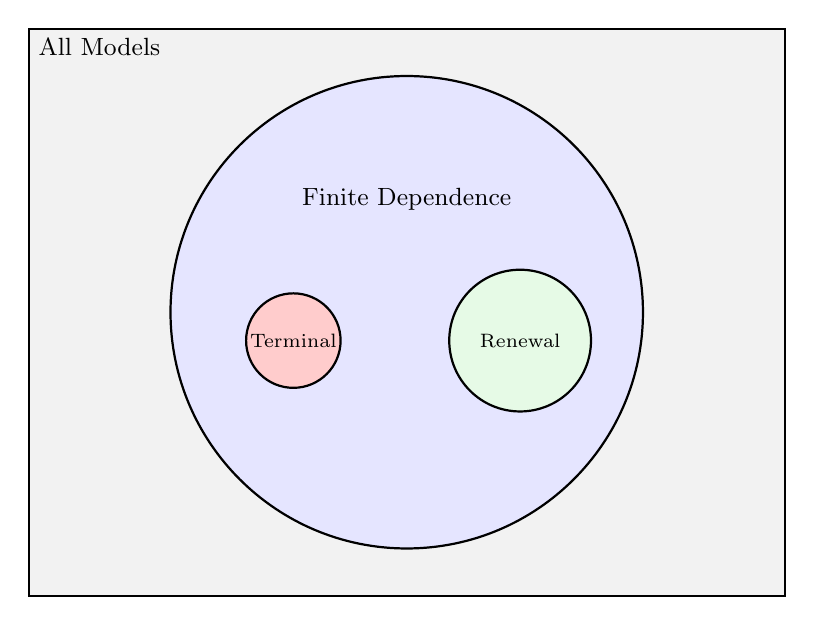
\begin{tikzpicture}[scale=1.2]
% Outer rectangle - all models
\draw[thick, fill=gray!10] (-4,-3) rectangle (4,3);
\node[anchor=north west] at (-4,3) {\small All Models};

% Large circle - finite dependence
\draw[thick, fill=blue!10] (0,0) circle (2.5cm);
\node at (0,1.2) {\small Finite Dependence};

% Left circle - terminal
\draw[thick, fill=red!20] (-1.2,-0.3) circle (0.5cm);
\node at (-1.2,-0.3) {\scriptsize Terminal};

% Right circle - renewal  
\draw[thick, fill=lightgreen] (1.2,-0.3) circle (0.75cm);
\node at (1.2,-0.3) {\scriptsize Renewal};

% Note: circles don't overlap (disjoint sets)
\end{tikzpicture}
\end{center}

Terminal and Renewal are \textit{disjoint} special cases

\end{frame}



\begin{frame}
State cancellation for Rust bus engine model:

\begin{center}
\begin{tabular}{cccc}
& $t$ & $t+1$ & $V_{t+2}$ \\[0.5em]
\midrule
\onslide<1->{
$v_{0t}(X_t)$: & (maintain) & (replace) & \\
& $X_t$ & $X_{t+1}$ & $0$ \\[2em]
}
\onslide<2->{
$v_{1t}(X_t)$: & (replace) & (replace) & \\
& $X_t$ & $0$ & $0$ \\
}
\end{tabular}
\end{center}

\bigskip

\onslide<3->{
When taking $v_{1t}(X_t) - v_{0t}(X_t)$, both paths lead to state $X_{t+2}=0$

\bigskip

$V_{t+2}$'s cancel, so only need $u_j(X_{t+1})$ and $\log(p_j(X_{t+1})$ terms---no backward recursion
}

\end{frame}





% Key difference: Arcidiacono = offer arrival then accept/reject; Ransom = location choice then lottery outcome

\begin{frame}
What if there is no renewal?
\bigskip\par
\onslide<2->{
Consider a simple model of labor supply:
\bigskip\par
}

\begin{itemize}
\itemsep1.5em
    \item<3-> $\mathcal{J}=\{\text{work},\text{home}\}$
    \item<4-> $X_t = \{\text{exper}_t,d_{t-1}\}$; no depreciation of $\text{exper}_t$ over time
    \item<5-> $u_j(X_t) = X_t \alpha_j$
    \item<6-> $\epsilon \overset{iid}{\sim}$ T1EV
\end{itemize}

\onslide<7->{
\bigskip\par
Can we get this model to satisfy finite dependence?
}
\end{frame}





\begin{frame}
State cancellation:

\begin{center}
\begin{tabular}{ccccc}
& $t$ & $t+1$ & $t+2$ & $V_{t+3}$ \\[0.5em]
\midrule
\onslide<1->{
$v_{ht}(X_t)$: & (home) & (work) & (home) & \\
& $\text{exper}_t$ & $\text{exper}_t$ & $\text{exper}_t+1$ & $\text{exper}_t+1$ \\
& $d_{t-1}$        & $d_{t}=h$ & $d_{t+1}=w$ & $d_{t+2}=h$ \\[2em]
}
\onslide<2->{
$v_{wt}(X_t)$: & (work) & (home) & (home) & \\
& $\text{exper}_t$ & $\text{exper}_t+1$ & $\text{exper}_t+1$ & $\text{exper}_t+1$ \\
& $d_{t-1}$        & $d_{t}=w$ & $d_{t+1}=h$ & $d_{t+2}=h$ \\
}
\end{tabular}
\end{center}
\bigskip\par

\onslide<3->{
When taking $v_{wt}(X_t) - v_{ht}(X_t)$, both paths lead to same $X_{t+3}$'s

\bigskip

$V_{t+3}$'s cancel, so only need $u_j(X_{t+1})$, $u_j(X_{t+2})$, $\log(p_j(X_{t+1})$ and $\log(p_j(X_{t+2})$
}

\end{frame}






\begin{frame}

\onslide<1->{
Earlier, I said, ``Also likely need additional assumptions about how states evolve''
\bigskip\par
}

\onslide<2->{
Key assumption for this model was no depreciation of labor market experience
\bigskip\par
}

\end{frame}



\begin{frame}

\onslide<1->{
Finite dependence can accommodate flexible models:
\bigskip\par
}

\begin{itemize}
\itemsep1.5em
    \item<2-> Arcidiacono, Aucejo, Maurel and Ransom (2025, JPE)
    \item<2->[]
    \begin{itemize}
    \itemsep1.5em
        \item<3-> White collar job offers, probabilistic graduation 
    \end{itemize}
    \item<4-> Ransom (2022, JHR)
    \item<4->[]
    \begin{itemize}
    \itemsep1.5em
        \item<5-> Employment lottery upon moving to a new city
    \end{itemize}
    \item<6-> Both weight different choice paths such that weights sum to 1
    \item<6->[]
    \begin{itemize}
    \itemsep1.5em
        \item<7-> Weights need not be in unit interval
    \end{itemize}
\end{itemize}

\end{frame}




\end{document}